\documentclass[a4paper&11pt]{article}
\usepackage{caption}
\usepackage{subcaption}
\usepackage{float}
\usepackage[caption = false]{subfig}
\usepackage{graphicx}

\newcommand{\subf}[2]{%
  {\small\begin{tabular}[t]{@{}c@{}}
  #1\\#2
  \end{tabular}}%
}  


\begin{document}
\section*{Appendix}

\subsection*{Simulation 1}
\subsubsection*{Erdos-Renyi Graphs}


\begin{table}[h]
\centering
\caption{My caption}
\label{my-label}
\resizebox{\textwidth}{!}{\begin{tabular}{c|c|c|c|c|c|c|c|c}
\hline
index & pn & order & size & density & cluster coefficient &diameter & nodes deg $\geq$ n & largest component \\ \hline
0& 0.01& 143& 107& 0.010538757017630258& 0.02097902097902098& inf& 0& 62\\ \hline 
1& 0.03& 143& 310& 0.030532847434255887& 0.027917032462487012& inf& 1& 142\\ \hline
 2& 0.05& 143& 482& 0.047473653107455924& 0.04904388540752172& 5& 4& 143\\ \hline
 3& 0.07& 143& 733& 0.07219541022357924& 0.06419614482140189& 4& 50& 143\\ \hline
 4& 0.09& 143& 913& 0.089924160346695564& 0.09865880287030333& 4& 94& 143\\ \hline
 5& 0.11& 143& 1089& 0.10725893824485373& 0.10842741064136702& 3& 120& 143\\ \hline
\end{tabular}}
\end{table}

\begin{figure}[h]
\centering
\begin{tabular}{|c|c|}
\hline
\subf{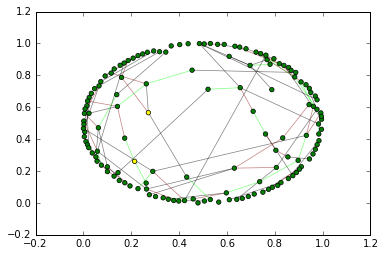
\includegraphics[width=60mm]{grapher01.png}}
     {}
&
\subf{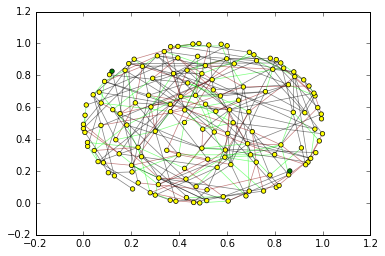
\includegraphics[width=60mm]{grapher03.png}}
     {}
\\
\hline
\subf{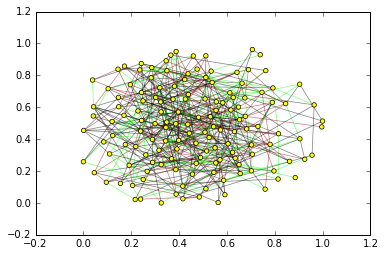
\includegraphics[width=60mm]{grapher05.png}}
     {}
&
\subf{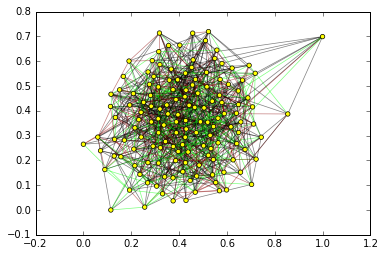
\includegraphics[width=60mm]{grapher09.png}}
     {}
\\
\hline
\end{tabular}
\caption{}
\end{figure}


\begin{figure}[h]
\centering
\begin{tabular}{|c|c|}
\hline
\subf{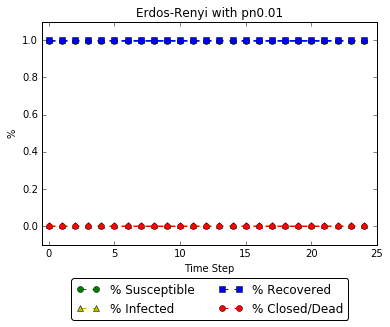
\includegraphics[width=60mm]{ploter01.png}}
     {}
&
\subf{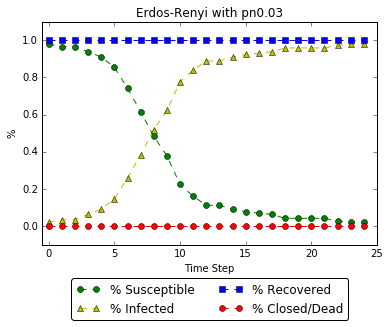
\includegraphics[width=60mm]{ploter03.png}}
     {}
\\
\hline
\subf{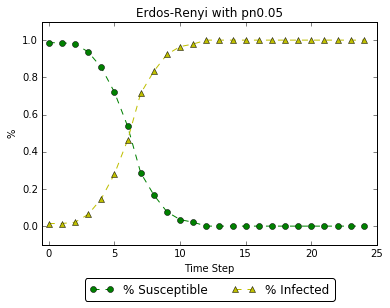
\includegraphics[width=60mm]{ploter05.png}}
     {}
&
\subf{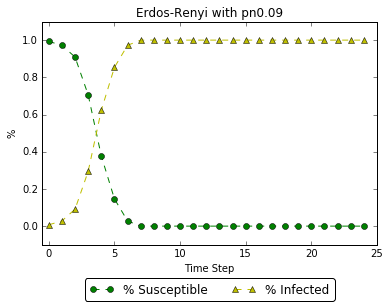
\includegraphics[width=60mm]{ploter09.png}}
     {}
\\
\hline
\end{tabular}
\caption{}
\end{figure}

\subsubsection*{Real Airport Graph and subgraphs}


\begin{center}
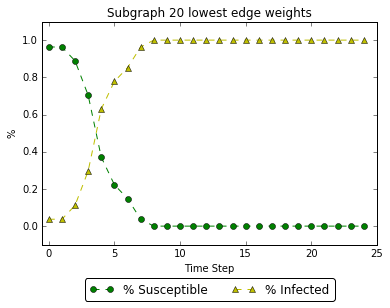
\includegraphics[width=13.7cm, height=8.2cm]{sublowestedgewsim1.png}
\begin{figure}[!h]
\caption{Here the caption.}
\end{figure}
\end{center}



\subsection*{Simulation 2}
\subsubsection*{Erdos-Renyi Graphs}


\begin{table}[h]
\centering
\caption{My caption}
\label{my-label}
\resizebox{\textwidth}{!}{\begin{tabular}{c|c|c|c|c|c|c|c|c}
\hline
index & pn & order & size & density & cluster coefficient &diameter & nodes deg $\geq$ n & largest component \\ \hline
0& 1& 143& 92& 0.0090613611740372312& 0.0& inf& 0& 57\\ \hline
1& 3& 143& 306& 0.030138875209297745& 0.0365028910483456& inf& 1& 141\\ \hline
2& 5& 143& 510& 0.050231458682162909& 0.03737385380742022& 5& 9& 143\\ \hline
3& 7& 143& 731& 0.071998424111100162& 0.06340691850770003& 4& 45& 143\\ \hline
4& 9& 143& 871& 0.085787451984635082& 0.07962630387817257& 4& 82& 143\\ \hline
5& 11& 143& 1156& 0.1138579730129026& 0.11439760465431766& 3& 126& 143\\ \hline
\end{tabular}}
\end{table}

\begin{figure}[h]
\centering
\begin{tabular}{|c|c|}
\hline
\subf{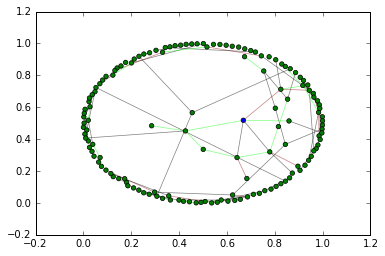
\includegraphics[width=60mm]{graphdie01.png}}
     {}
&
\subf{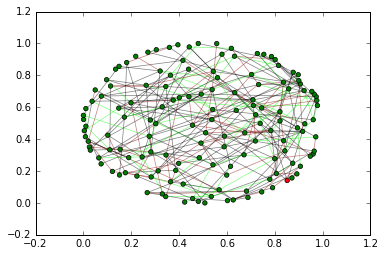
\includegraphics[width=60mm]{graphdie03.png}}
     {}
\\
\hline
\subf{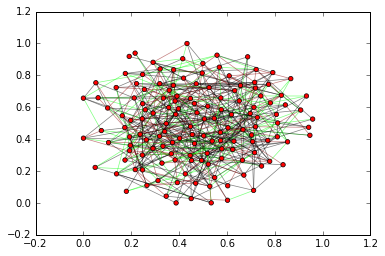
\includegraphics[width=60mm]{graphdie05.png}}
     {}
&
\subf{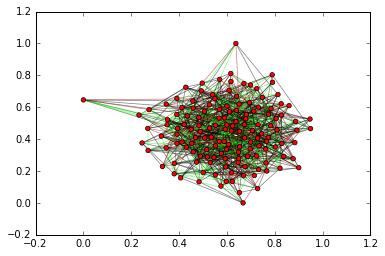
\includegraphics[width=60mm]{graphdie09.png}}
     {}
\\
\hline
\end{tabular}
\caption{}
\end{figure}

\begin{figure}[h]
\centering
\begin{tabular}{|c|c|}
\hline
\subf{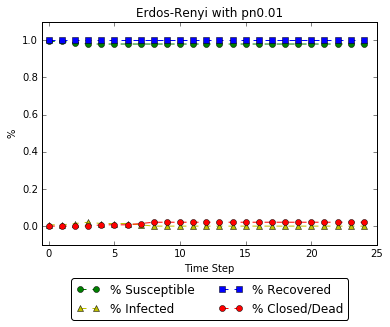
\includegraphics[width=60mm]{ploterdie01.png}}
     {}
&
\subf{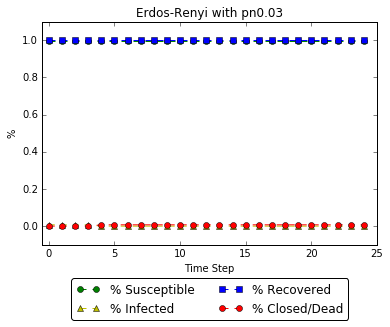
\includegraphics[width=60mm]{ploterdie03.png}}
     {}
\\
\hline
\subf{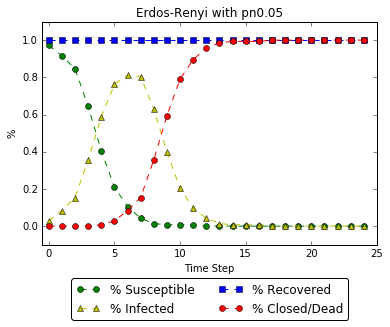
\includegraphics[width=60mm]{ploterdie05.png}}
     {}
&
\subf{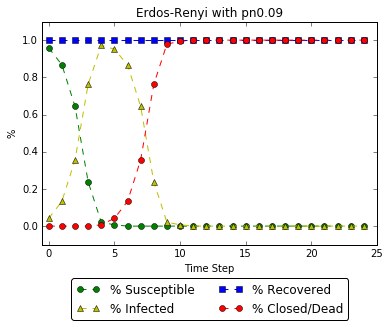
\includegraphics[width=60mm]{ploterdie09.png}}
     {}
\\
\hline
\end{tabular}
\caption{}
\end{figure}

\subsection*{Simulation 3}

\begin{table}[h]
\centering
\caption{My caption}
\label{my-label}
\resizebox{\textwidth}{!}{\begin{tabular}{c|c|c|c|c|c|c|c|c}
\hline
index & pn & order & size & density & cluster coefficient &diameter & nodes deg $\geq$ n & largest component \\ \hline
0& 1& 143& 91& 0.0089628681177976958& 0.002564102564102564& inf& 0& 40\\ \hline
1& 3& 143& 298& 0.029350930759381465& 0.01908091908091909& inf& 0& 141\\ \hline
2& 5& 143& 501& 0.049345021176007094& 0.041219347862704495& 5& 4& 143\\ \hline
3& 7& 143& 710& 0.069930069930069935& 0.07645401926561934& 4& 36& 143\\ \hline
4& 9& 143& 892& 0.087855806165665323& 0.09174894803128791& 4& 85& 143\\ \hline
5& 11& 143& 1103& 0.10863784103220724& 0.10304055495417155& 3& 125& 143\\ \hline
\end{tabular}}
\end{table}

\subsubsection*{Erdos-Renyi Graphs}
\begin{figure}[h]
\centering
\begin{tabular}{|c|c|}
\hline
\subf{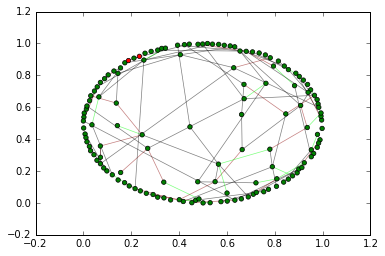
\includegraphics[width=60mm]{graphrec01.png}}
     {}
&
\subf{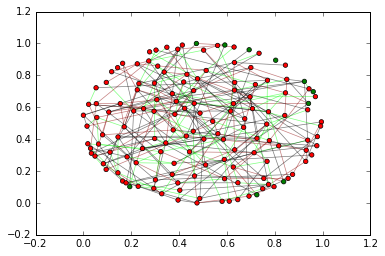
\includegraphics[width=60mm]{graphrec03.png}}
     {}
\\
\hline
\subf{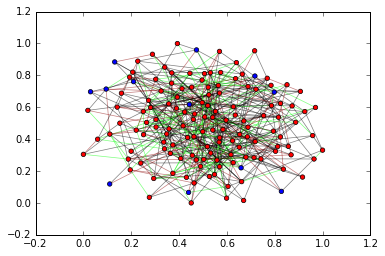
\includegraphics[width=60mm]{graphrec05.png}}
     {}
&
\subf{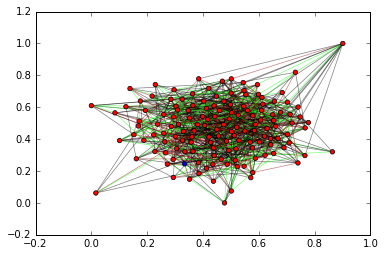
\includegraphics[width=60mm]{graphrec09.png}}
     {}
\\
\hline
\end{tabular}
\caption{}
\end{figure}

\begin{figure}[h]
\centering
\begin{tabular}{|c|c|}
\hline
\subf{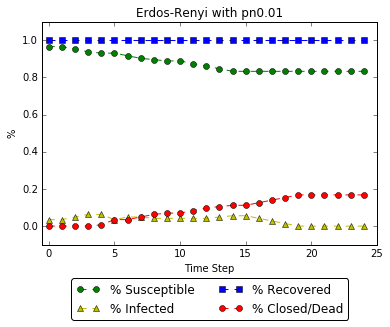
\includegraphics[width=60mm]{plotrec01.png}}
     {}
&
\subf{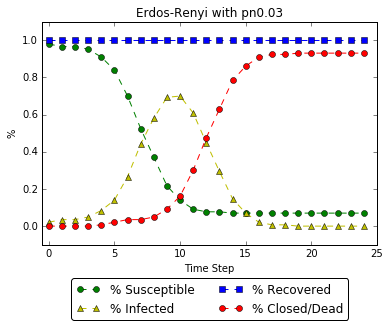
\includegraphics[width=60mm]{plotrec03.png}}
     {}
\\
\hline
\subf{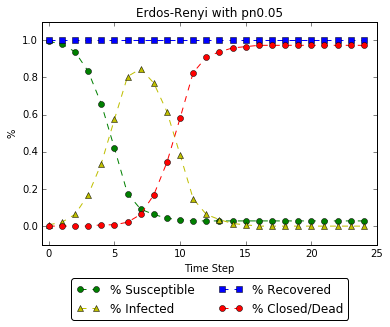
\includegraphics[width=60mm]{plotrec05.png}}
     {}
&
\subf{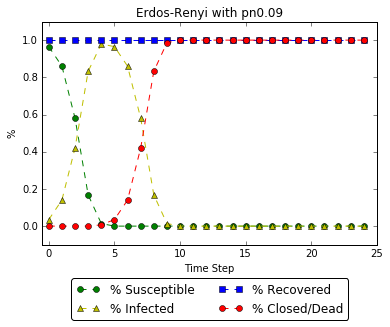
\includegraphics[width=60mm]{plotrec09.png}}
     {}
\\
\hline
\end{tabular}
\caption{}
\end{figure}

\end{document}